\documentclass[12pt, oneside]{article}
\usepackage[letterpaper, margin=1in, headsep=0.5in]{geometry}
\usepackage[english]{babel}
\usepackage[utf8]{inputenc}
\usepackage{amsmath}
\usepackage{amsfonts}
\usepackage{amssymb}
\usepackage{tikz}
\usetikzlibrary{quotes, angles}
\usepackage{graphicx}
%\usepackage{pgfplots}
%\pgfplotsset{width=10cm,compat=1.9}
%\usepgfplotslibrary{statistics}
%\usepackage{pgfplotstable}
%\usepackage{tkz-fct}
%\usepackage{venndiagram}

\usepackage{fancyhdr}
\pagestyle{fancy}
\fancyhf{}
\rhead{\thepage \\Name: \hspace{1.5in}.\\}
\lhead{BECA / Dr. Huson / 10th Grade Geometry\\* 16 November 2018}

\renewcommand{\headrulewidth}{0pt}

\begin{document}
\subsubsection*{Do Now: Graphing the features of a parallelogram}
  \begin{enumerate}

\item Given parallelogram $SNOW$ with $S(2,1),N(7,1),O(10,5),W(5,5)$}
    \begin{enumerate}
      \item Sketch $SNOW$, labeling the vertices.\\
        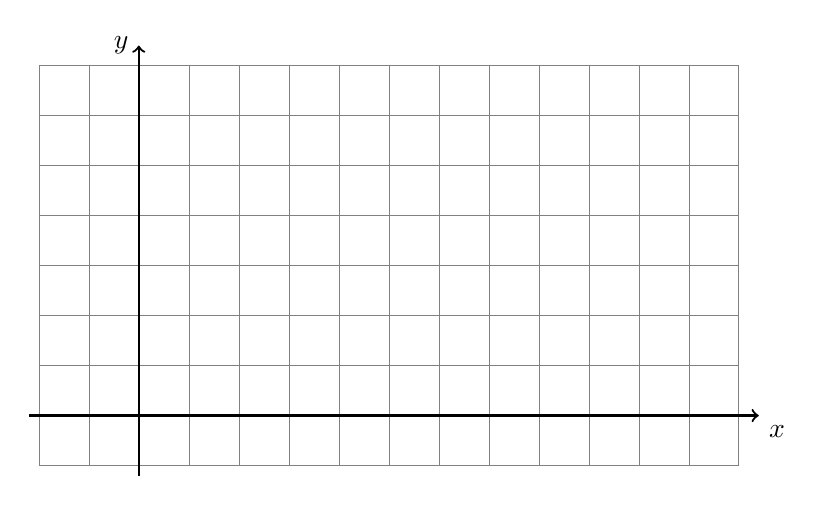
\begin{tikzpicture}[scale=.635]
          \draw [help lines] (-2,-1) grid (12,7);
          \draw [thick, ->] (-2.2,0) -- (12.4,0) node [below right] {$x$};
          \draw [thick, ->] (0,-1.2)--(0,7.4) node [left] {$y$};
        \end{tikzpicture}
      \item Find the area of the parallelogram.\vspace{3cm}
      \item Find the length of each side of the parallelogram.\vspace{5cm}
      \item Find the slopes of the diagonals, $\overline{SO}$ and $\overline{NW}$.\vspace{3.5cm}
      \item Are the diagonals parallel, perpendicular, or neither? Justify your answer.
  \end{enumerate}

\end{enumerate}
\end{document}
